\chapter{Implementierung}
\label{chp:implementierung}

In diesem Kapitel wird die gesamte Systemumgebung um das Steuerelement in Form eines Raspberry Pi beschrieben und erläutert.
Die gesamte Implementierung der Steuerungsskripts erfolgt in Python und wird sinnvoll in Module unterteilt.
Der Quelltext zum gesamten Projekt wird auf GitHub veröffentlicht.

Insgesamt werden vier Module implementiert, die alle diskrete Funktionalitäten des Modells abdecken: Die Funktionen zur Motoransteuerung sind im Modul \texttt{Actuator} implementiert. 
Für die Bilderkennung der Wasserobjekte auf einem Kamera-Feed der verwendeten Kamera (Details siehe Abschnitt \ref{sec:inst_konf_kamera}) ist das Modul \texttt{Camera} entwickelt worden.
Die programmierten Skripte für Sprachein- und -ausgabe befinden sich respektive in den Modulen \texttt{Voice\_Recognition} und \texttt{Voice\_Output}.
Koordiniert wird die auf diesen vier Modulen basierende Roversteuerung durch das Skript \texttt{rover.py}.
In der Konfigurationsdatei \texttt{config.py} werden Variablen zur globalen Nutzung zentral deklariert und mit passenden Werten initialisiert.

Um die gleichzeitige Sprach- und Objekterkennung zu ermöglichen, erzeugt das Hauptskript zwei Threads, die eine quasi-zeitgleiche Verarbeitung der entsprechenden Funktionen ermöglichen \cite{donat2018, yamanoor2017}.
Die Funktion, welche im Thread für die Wassererkennung aufgerufen wird, nimmt als Argument eine Callback-Funktion entgegen.
Hier wird die Funktion \texttt{water\_found} des Moduls \texttt{Voice\_Output} übergeben, sodass bei jeder Erkennung eines Wasser-Objektes der Text \enquote{Water found} ausgegeben wird.
Die Ausgabefunktionalitäten der Software beruhen auf der \texttt{pyttsx3}-Bibliothek, welche umfangreiche Text-to-speech-Funktionen und Unterstützung für verschiedene Synthesizer bereitstellt.
Als Sprach-Synthesizer wird hier wegen seiner Leichtgewichtigkeit und Kompatibilität zu Raspbian \textit{eSpeak} \cite{molloy2016} genutzt.
Die Spracherkennung ruft entsprechende Funktionen zur Motorsteuerung nach der Erkennung von Eingabebefehlen direkt auf und benötigt demnach keine Callback-Funktion.
Zur Erkennung der Sprachbefehle kann \textit{PocketSphinx} genutzt werden.
Mit einigem Training könne dieses gute Resultate produzieren \cite[vgl.][S. 644]{molloy2016}, also eine zuverlässige Erkennung der Sprachbefehle auch offline ermöglichen.
Für die Dauer der Entwicklung wird die Spracherkennung mithilfe eines frei zugänglichen Online-Dienstes von Google durchgeführt, da hier der Trainingsaufwand entfällt und die Erkennung schnell und weitestgehend präzise geschieht.
Allerdings ist dieser entsprechend nur erreichbar, wenn eine aktive Internetverbindung mit ausreichend geringer Latenz besteht.
Darüber hinaus kann für \textit{PocketSphinx} ein selbst-definierter Satz zu erkennender Worte (zum Beispiel die Steuerbefehle laut Spezifikation) festgelegt werden, wodurch viele Resultate kategorisch ausgeschlossen und die Erkennung beschleunigt werden kann.

Die gesamte Python-Entwicklung ist mithilfe der \texttt{setup.py} als zusammenhängendes Paket aufgesetzt worden.
So kann innerhalb einer virtuellen Umgebung (hier \texttt{venv} genannt) von jedem Modul auf jedes andere zugegriffen werden.
Hinweise und Anweisungen zum Setup und der Aktivierung einer virtuellen Python-Umgebung sind in \cite{langtangen2016} festgehalten.

Bezüglich der Motoransteuerung hat sich gezeigt, dass mindestens $25\ \%$ der von der Hardware erlaubten Motorleistung abgerufen werden sollten.
Bei Testfahrten sind teilweise Steuersignale bei niedrigerer Leistungsangabe nicht vollständig übertragen worden, vermutlich aufgrund einer zu niedrig angelegten Spannung am BrickPi.
Darüber hinaus führt ein zu hohes Gewicht des Rover-Korpus dazu, dass die Motoren mit höherer Leistungsstufe laufen müssen.
Ansonsten können sie unter Umständen kein ausreichendes Drehmoment aufbauen, um den Rollwiderstand der Räder zu überwinden.

\begin{figure*}
	\centering
	\begin{subfigure}[t]{0.4\textwidth}
		\centering
		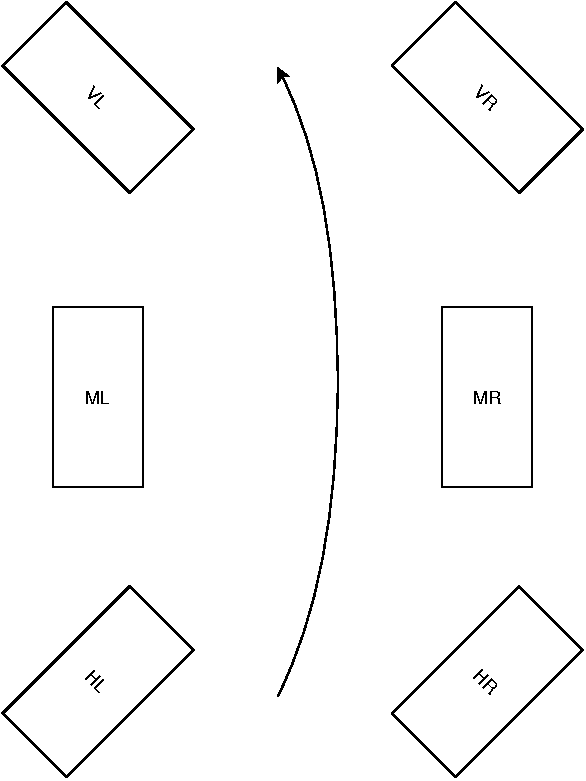
\includegraphics[height=4cm]{../Images/kurve.pdf}
		\caption{Klassische Kurvenfahrt bei einer Zweiachslenkung}
		\label{subfig:kurve}
	\end{subfigure}
	~
	\begin{subfigure}[t]{0.4\textwidth}
		\centering
		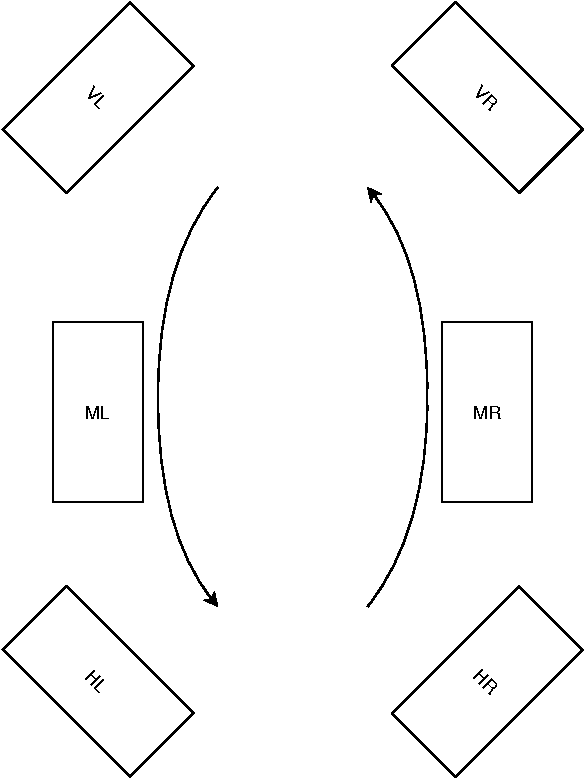
\includegraphics[height=4cm]{../Images/rotate.pdf}
		\caption{Rotation durch Rautenanordnung der Räder und entgegengesetzten Antrieb beider Seiten}
		\label{subfig:rotation}
	\end{subfigure}
	\caption{Varianten einer Linkskurve beziehungsweise -rotation beim genutzten Antriebskonzept}
	\label{fig:moveleft}
\end{figure*}

Mangels Achsendifferentialen wird statt einer üblichen Kurvenfahrt wie in Abbildung \ref{subfig:kurve} dargestellt eine Rotation des Rovers auf der Stelle in beide Richtungen implementiert.
Abbildung \ref{subfig:rotation} zeigt die dafür angestrebte Anordnung der Räder in Winkeln von jeweils $\pm45\degree$ zur Fahrtrichtung und die jeweilige Antriebsrichtung der Räder -- beispielsweise werden für eine Linksrotation die drei linken Räder rückwärts und die drei rechten vorwärts angetrieben.
So lässt sich ein Auseinanderdriften der einzelnen Räderpaare (vorn, Mitte, hinten) weitestgehend vermeiden.
Trotzdem werden zum Abschluss einer Rotationsbewegung die lenkbaren Räder für eine kurze Strecke um $15\degree$ zur Fahrtrichtungsachse gerichtet, da sich dieses Auseinanderdriften auch bei der Rotation nicht vollständig vermeiden lässt.

\section{Installation und Konfiguration Raspberry Pi}
\label{sec:inst_konf_raspi}

Die Steuerung des Mars-Rover-Modells erfolgt zentral über einen Raspberry Pi 3 Model B Plus (Revision 1.3).
Auf diesem ist die Debian-basierte Distribution Raspbian for Robots der US-amerikanischen Firma Dexter Industries installiert worden.
Dieses Betriebssystem enthält standardmäßig viele vorinstallierte Anwendungen und Treiber für den Einsatz des Raspberry Pi zur Steuerung von Robotern.
Zusätzlich sind hier standardmäßig \acf{ssh} und \acf{vnc} Server installiert und aktiviert, sodass über das Netzwerk auch auf einen Pi, der in einem Roboter verbaut ist, zugegriffen werden kann \cite{donat2018, mcmanus2017}.
Insbesondere sind alle benötigten Bibliotheken zur Nutzung der zusätzlichen Platine BrickPi 3 vorinstalliert und -konfiguriert.
Der BrickPi ist ebenfalls ein Produkt von Dexter Industries und stellt eine Schnittstelle zwischen den verschiedenen LEGO-Mindstorms-Sensoren und -Motoren zum Raspberry Pi bereit.
Er ging 2013 aus einer enorm erfolgreichen Kickstarter-Kampagne hervor \cite{barnes2015} und ist seither weiterentwickelt worden, sodass in diesem Projekt der BrickPi 3 (2017) genutzt werden kann.
Die Platine fungiert dabei auch als Stromquelle für diese sowie für den Raspberry Pi selbst und muss dazu, ähnlich einer \acf{hat}, lediglich auf dessen Pins für \acf{gpio} aufgesteckt werden.
Da jeder BrickPi nur über vier Ausgänge zum Betrieb von EV3-Motoren verfügt, ist der gleichzeitige Einsatz von drei BrickPis nötig, um die zehn Motoren des Modells anzutreiben.
Dabei kann jedes der sechs Räder separat durch einen Motor angetrieben sowie die äußeren vier Räder einzeln gelenkt werden.
Eine Lenkung der mittleren Räder ist zum aktuellen Zeitpunkt nicht notwendig, kann aber problemlos über die verbleibenden beiden Ports der BrickPis ergänzt werden, beispielsweise um seitliche Fahrten zu ermöglichen.

\begin{figure} % TODO: "vorn" durch "vorne" ersetzen!
	\centering
	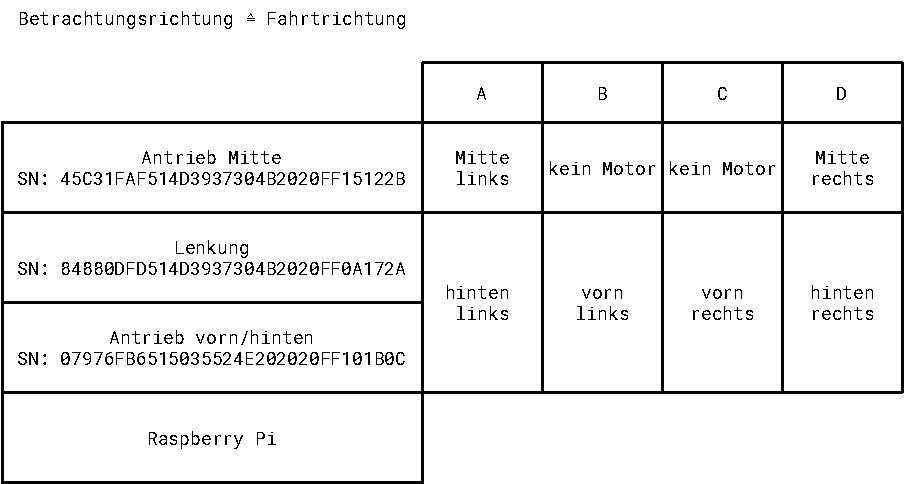
\includegraphics[width=0.8\textwidth]{../Images/brickpiconfig.pdf}
	\vspace{0.5em}
	\parbox[c]{0.8\linewidth}{\footnotesize
		\centering
		\vspace{1em}
		Quelle: eigene Darstellung
	}
	\caption{Belegung der Steuerungsausgänge zu den einzelnen Motoren an den drei BrickPis des Steuergerätes}
	\label{fig:brickpistack}
\end{figure}

In Abbildung \ref{fig:brickpistack} ist die standardmäßige Belegung der drei BrickPis sowie deren Seriennummern dargestellt.
Die Spalten \texttt{A} bis \texttt{D} entsprechen den Motorsteuerausgängen \texttt{MA} bis \texttt{MD} des BrickPi 3.
Eine Übersicht über dessen verschiedene Anschlüsse im Einzelnen ist der Vollständigkeit halber in Abbildung \ref{fig:brickpi3ports} abgebildet.
Die Bezeichnungen der Motoren anhand ihrer Richtung (vorn, hinten, links, rechts) sind dabei unter der Voraussetzung, dass der Rover in Fahrtrichtung betrachtet wird, zutreffend.

\begin{figure}
	\centering
	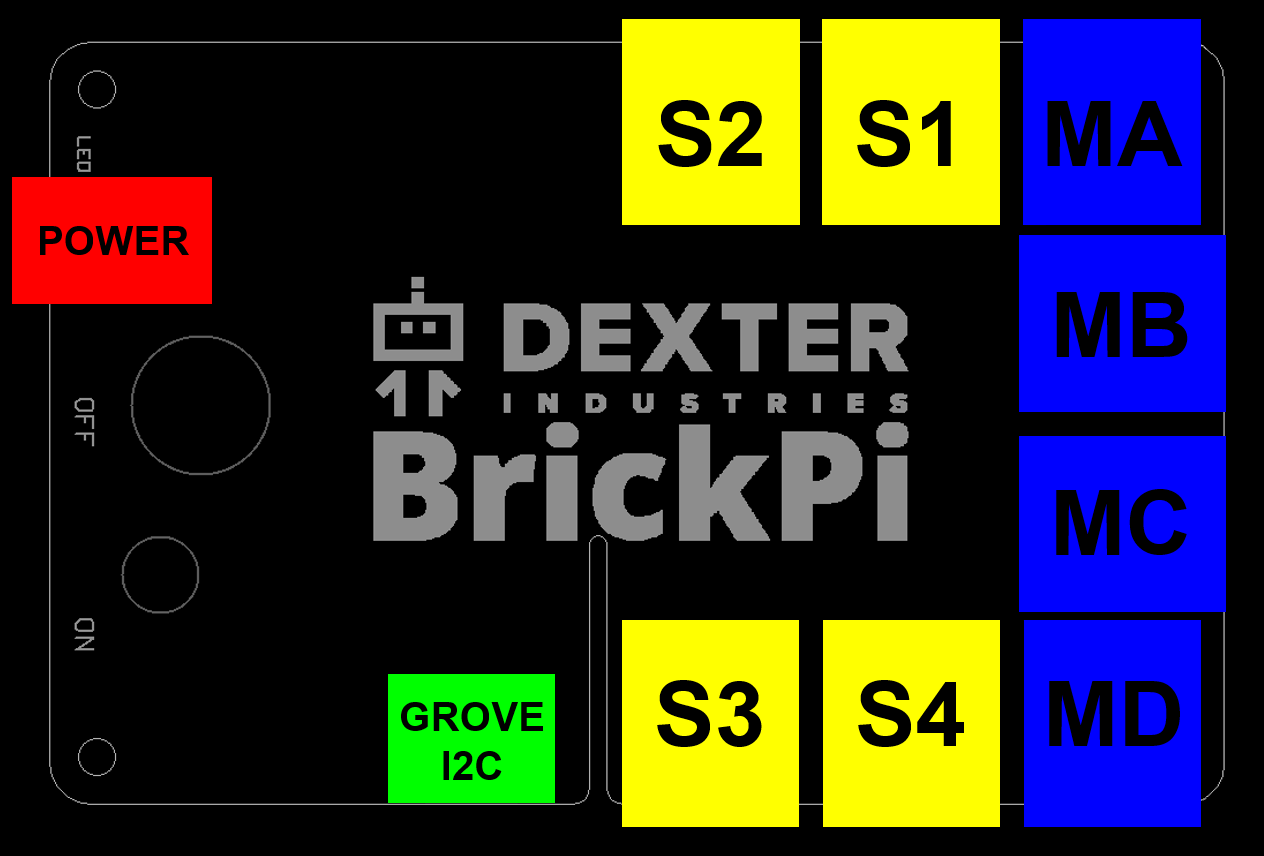
\includegraphics[width=0.5\textwidth]{../Images/BrickPi3-Port-Layout.png}
	\vspace{0.5em}
	\parbox[c]{0.8\linewidth}{\footnotesize
		\centering
		\vspace{1em}
		Quelle: \cite{dexter2017}
	}
	\caption{Belegung der Ein- und Ausgänge eines einzelnen BrickPi 3}
	\label{fig:brickpi3ports}
\end{figure}

Um die Stromversorgung sicherzustellen, werden drei Powerbanks (siehe Abbildung \ref{fig:powerbank}) mit einer Gesamtkapazität von $60{,}3\ Ah$ und einem Gesamtgewicht von $1251\ g$ im Korpus des Rovers untergebracht.
Der Raspberry Pi selbst wird durch die BrickPis über seine \acs{gpio}-Pins mit Energie versorgt \cite{cole2013} und benötigt entsprechend keine eigene Stromquelle.

\begin{wrapfigure}{l}{0.25\textwidth}
	\centering
	\includegraphics[width=0.9\linewidth]{../Images/powerbank.png}
	\vspace{0.5em}
	\parbox[c]{0.8\linewidth}{\footnotesize
		\centering
		\vspace{1em}
		Quelle: eigene Aufnahme
	}
	\captionsetup{format=plain}
	\caption{Powerbank der Firma XT Power, die zur Stromversorgung genutzt wird}
	\label{fig:powerbank}
\end{wrapfigure}

Zu beachten ist, dass beim Einschalten der drei BickPis über die jeweiligen Schalter einzelne Platinen unter Umständen die Präsenz eines Eingangsstroms nicht feststellen (können).
Es hat sich jedoch gezeigt, dass durch wiederholtes Aus- und Wiedereinschalten der BrickPis ein Zustand erreicht werden kann, in dem alle mit Strom versorgt sind.
Zu erkennen ist dies an blinkenden, orangefarbenen Status-Leuchtdioden neben den Schaltern.

Weiterhin führt ein Leerlauf des Systems gelegentlich dazu, dass sich die bereitgestellten Powerbanks bei vermeintlicher Nichtbenutzung selbst abschalten.
Dadurch ist ein BrickPi nicht mehr mit ausreichender Spannung versorgt, um die Motoren anzutreiben.
Das Gesamtsystem bleibt aber durch die anderen beiden Powerbanks mit Strom versorgt.
Wird eine der Powerbanks durch eines der Batteriepacks aus dem Lieferumfang des BrickPi (dargestellt in Abbildung \ref{fig:batteriepack}) mit acht AA-Batterien ersetzt, steht jederzeit an allen Platinen ausreichend Spannung und Strom bereit, um die Motoren zu betreiben.

\begin{figure}
	\centering
	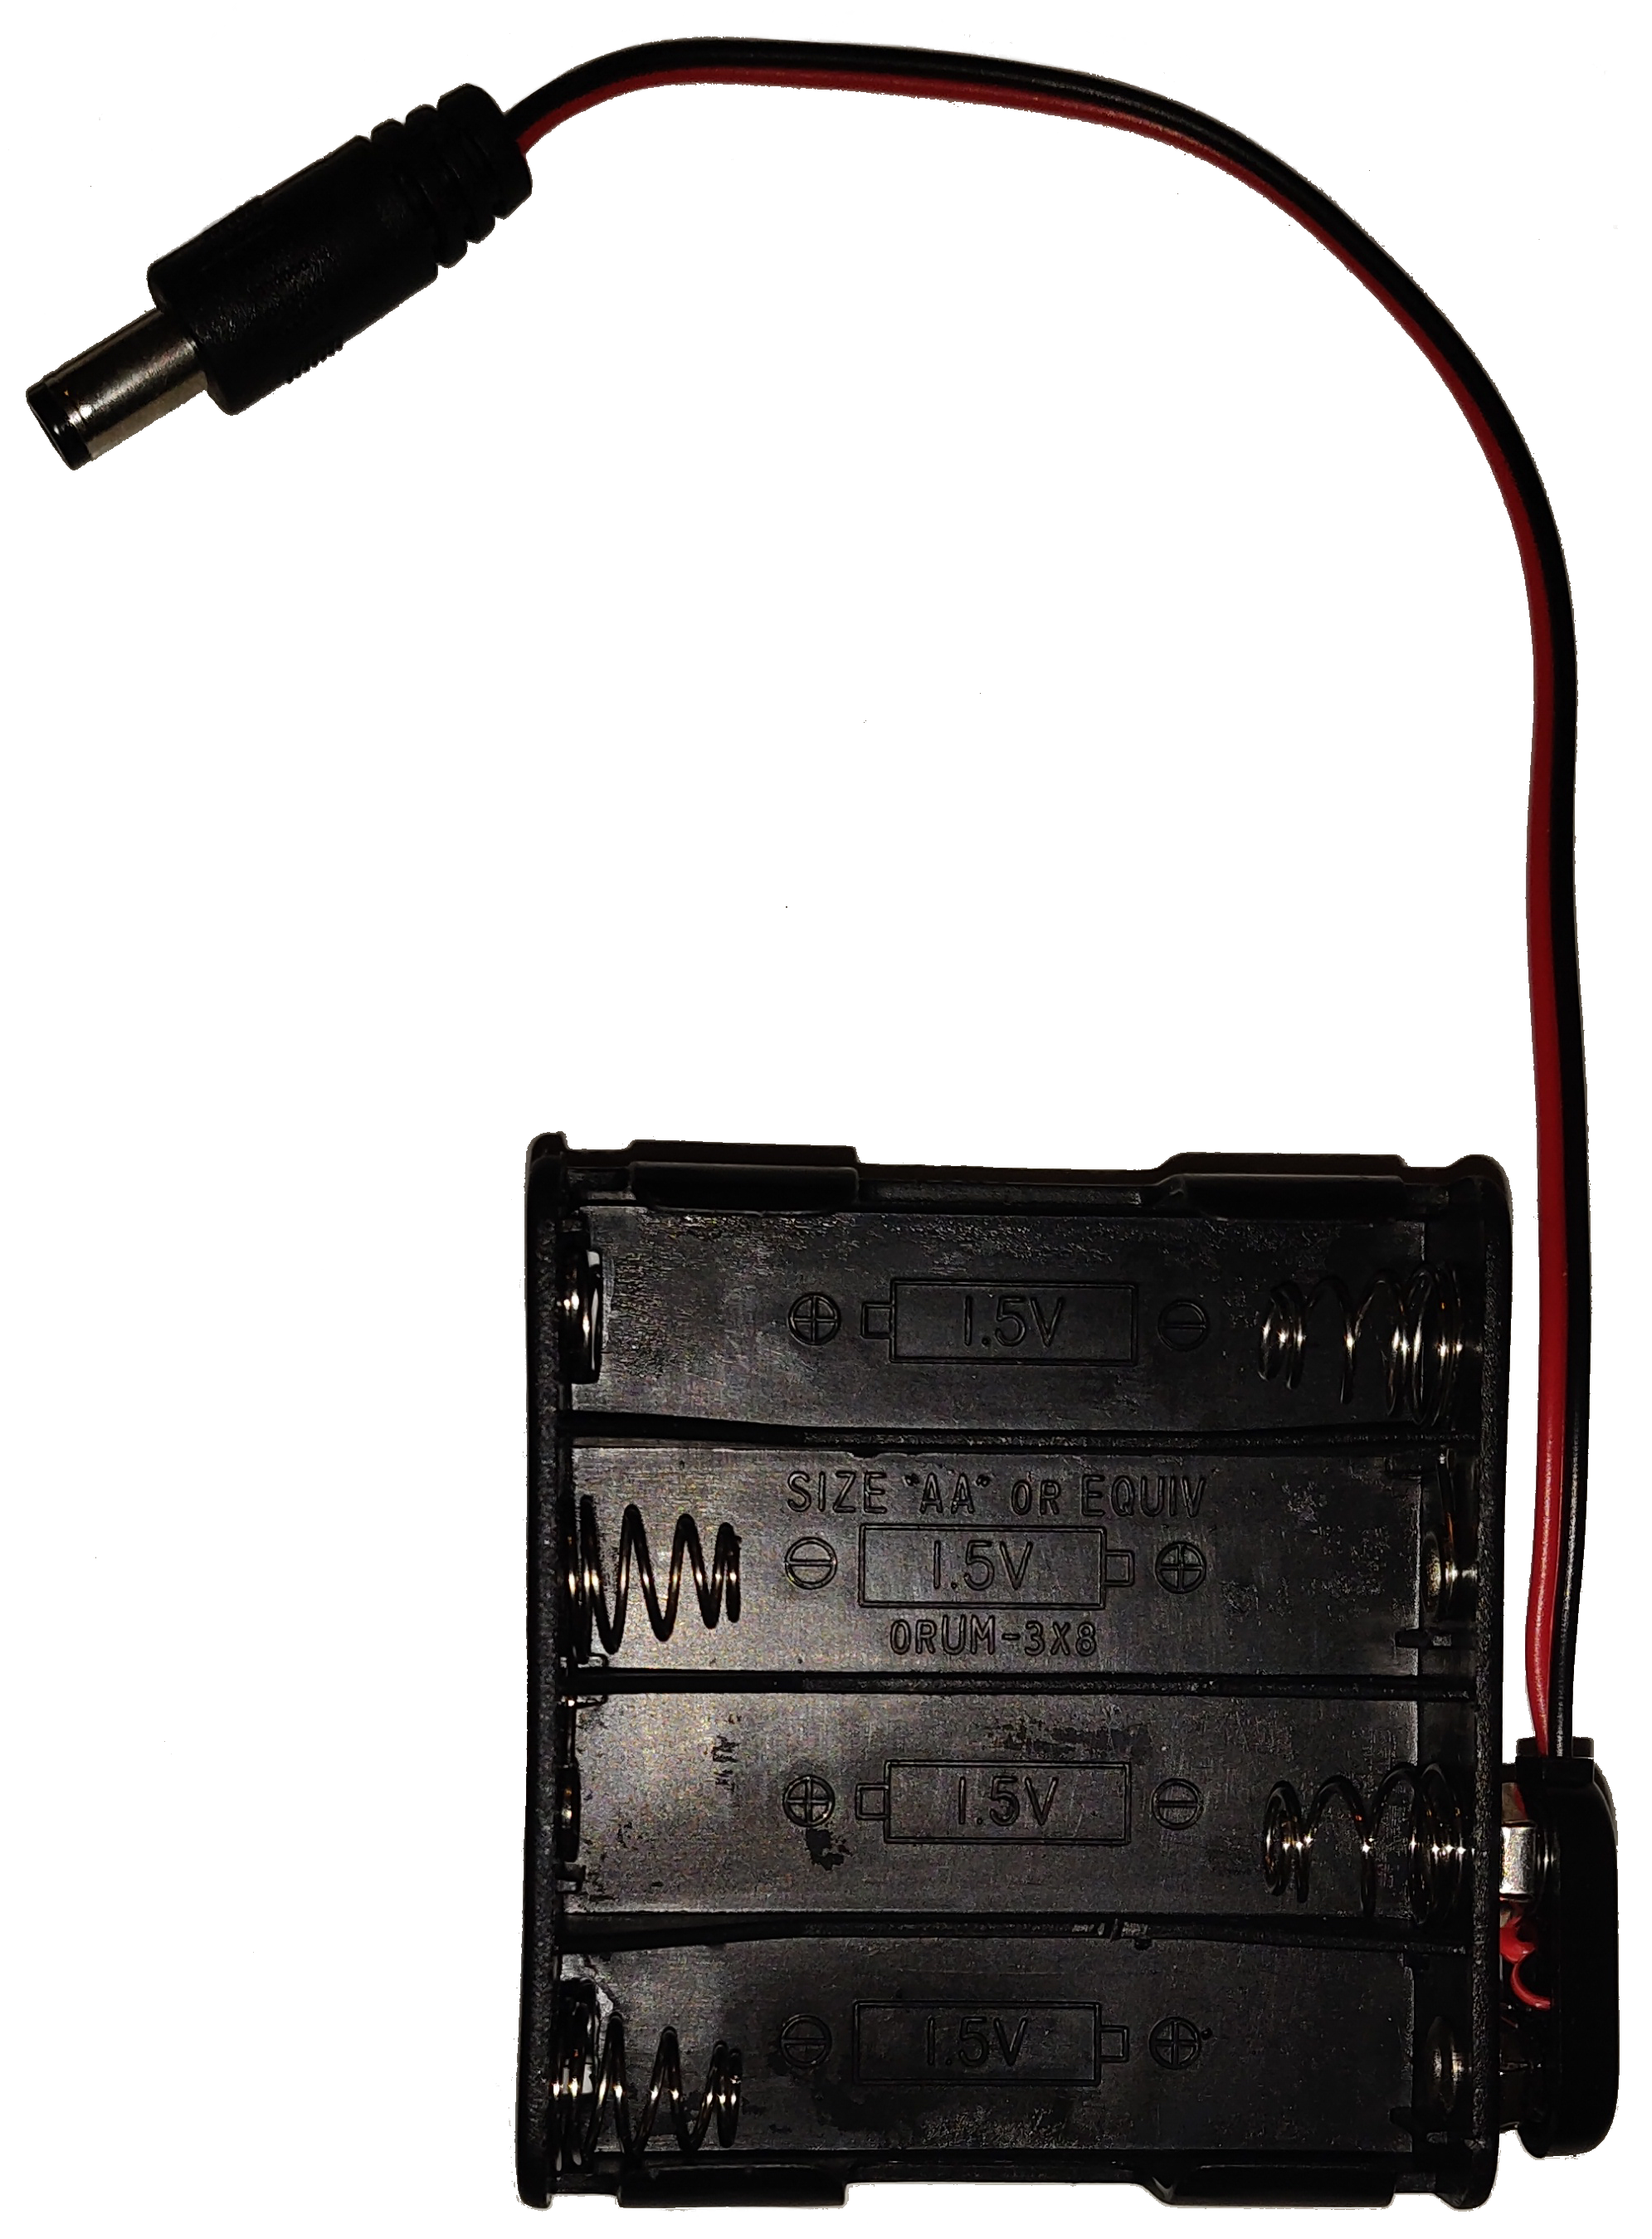
\includegraphics[angle=90,width=0.5\textwidth]{../Images/batteriepack.png}
	\vspace{0.5em}
	\parbox[c]{0.8\linewidth}{\footnotesize
		\centering
		\vspace{1em}
		Quelle: eigene Aufnahme
	}
	\caption{Alternative zur Powerbank: Batteriepack aus dem Lieferumfang des BrickPi}
	\label{fig:batteriepack}
\end{figure}

Für die Sprachein- und -ausgabe wird eine USB-Soundkarte angeschlossen, die jeweils eine $3{,}5$-mm-Klinkenbuchse für Lautsprecher und Mikrofon bereitstellt.
Die Konfiguration geschieht über die \acf{alsa} Utilities -- die unter Raspbian vorinstallierten Soundtreiber für den Raspberry Pi.
Neben dem Onboard-Sound über den Klinkenausgang des Raspberry Pi unterstützen diese auch die digitale Ausgabe über \acf{hdmi} sowie die genutzte Soundkarte über USB. \cite{molloy2016}

\begin{figure}
	\centering
	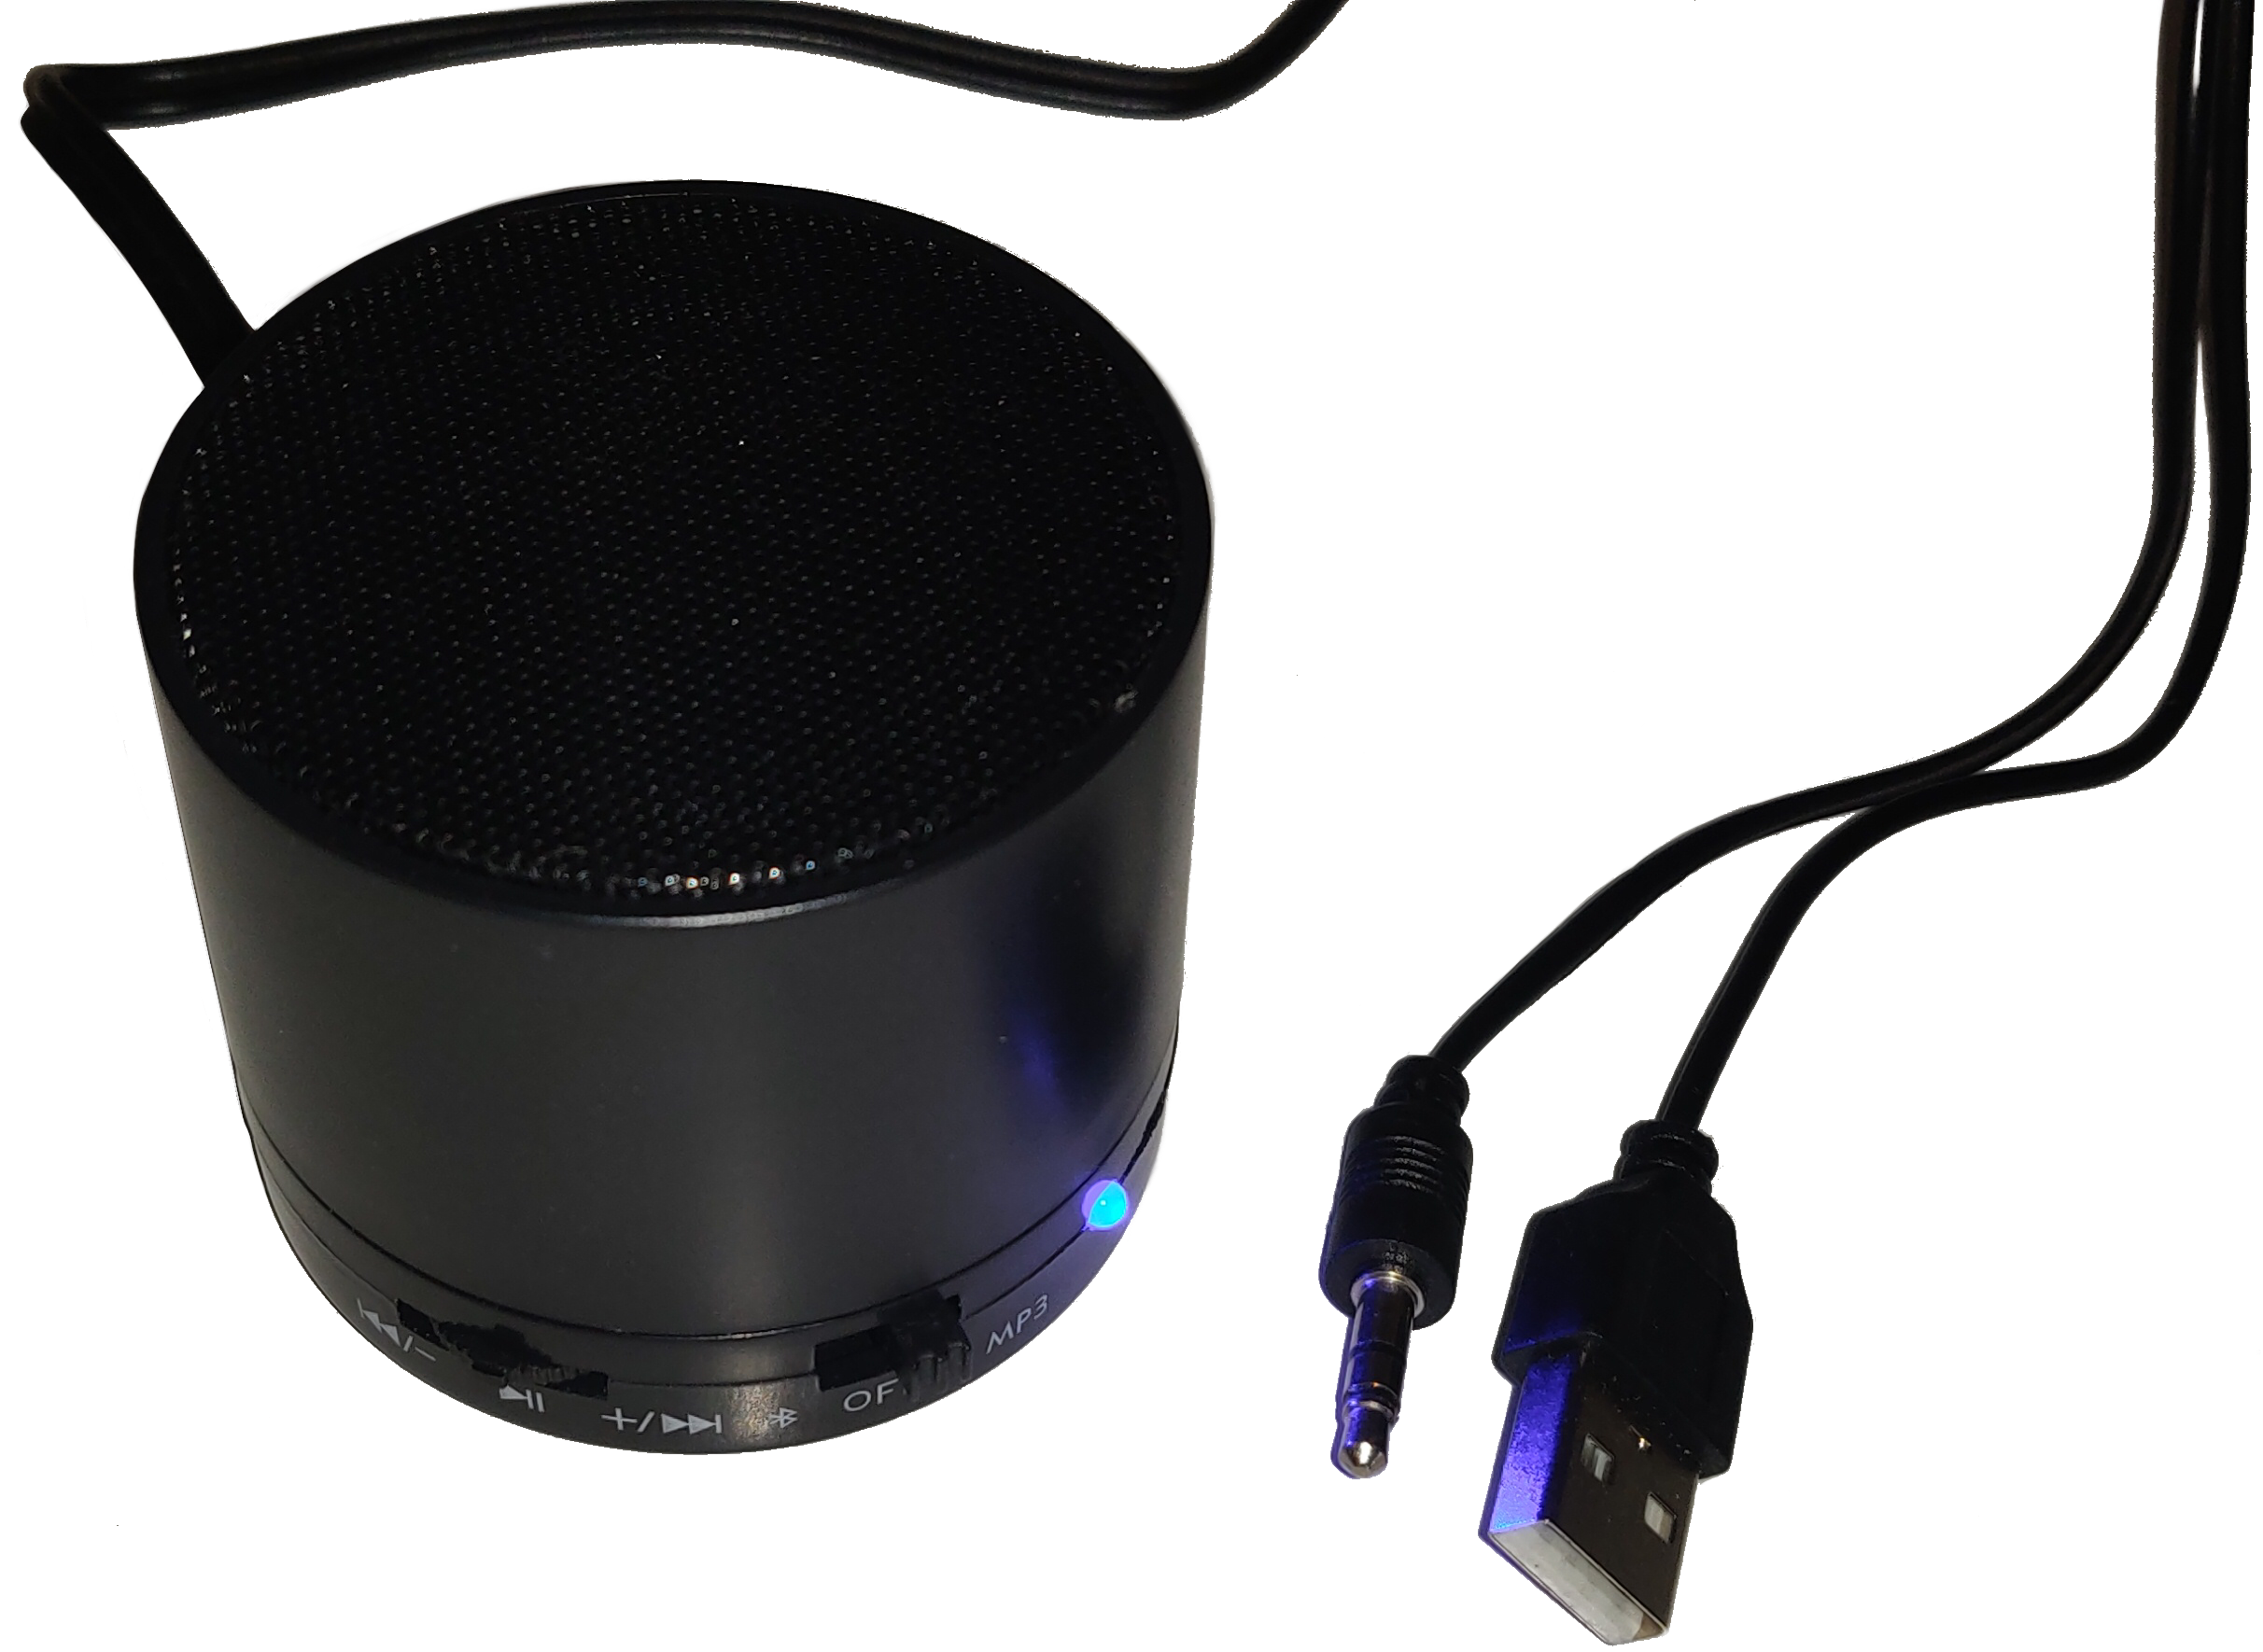
\includegraphics[width=0.5\textwidth]{../Images/lautsprecher.png}
	\vspace{0.5em}
	\parbox[c]{0.8\linewidth}{\footnotesize
		\centering
		\vspace{1em}
		Quelle: eigene Aufnahme
	}
	\caption{Für die Sprachausgabe genutzter Lautsprecher (Inspirion GmbH)}
	\label{fig:lautsprecher}
\end{figure}

Die Ausgabe geschieht dabei mithilfe eines Bluetooth-Lautsprechers (vertrieben durch die Inspirion GmbH), welcher über einen eigenen Akku verfügt und mittels Klinke an die oben genannte Soundkarte angeschlossen wird.
Der genutzte Lautsprecher ist in Abbildung \ref{fig:lautsprecher} dargestellt.

\section{Installation und Konfiguration Kamera}
\label{sec:inst_konf_kamera}

Für die Videoeingabe wird die originale Raspberry Pi Camera V2 genutzt.
Diese nutzt den CMOS-Sensor Sony IMX219 mit einer Auflösung von bis zu 8 Megapixeln \cite{pagnutti2017} und kann mithilfe eines mitgelieferten Flachbandkabels an das \acf{csi} des Raspberry Pi angeschlossen werden \cite{halfacree2019}.
Die Aufnahmen erfolgen mit einer reduzierten Auflösung von $1280 \times 720$ Pixeln, um eine Frequenz von $60\ Hz$ zu ermöglichen. 
So ist sichergestellt, dass Wasserobjekte auch während der Fahrt gut erkannt werden können.
Alternativ kann eine Frequenz von $90\ Hz$ bei geringerer Auflösung ($640 \times 480$ oder niedriger) erreicht werden \cite{halfacree2019}.
Allerdings zeigte sich während der Entwicklung, dass bei den oben genannten Parametern die Erkennung am präzisesten funktioniert.

\begin{wrapfigure}{l}{0.25\textwidth}
	\centering
	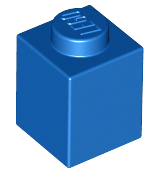
\includegraphics[width=0.9\linewidth]{../Images/3005.png}
	\vspace{0.5em}
	\parbox[c]{0.8\linewidth}{\footnotesize
		\centering
		\vspace{1em}
		Quelle: \url{https://www.bricklink.com/v2/catalog/catalogitem.page?P=3005\&C=7}
	}
	\captionsetup{format=plain}
	\caption{Blauer LEGO-Stein 3005}
	\label{fig:lego3005}
\end{wrapfigure}

Die Objekterkennung für Wasserobjekte erfolgt mithilfe der Programmbibliotheken picamera und OpenCV.
Erstere stellt eine Schnittstelle zwischen der Raspberry-Pi-Kamera und Python zur Verfügung \cite{cox2014}.
Letztere Bibliothek ermöglicht die Echtzeitauswertung der Kamerabilder \cite{pajankar2015}:
Die Objekte werden auf Basis ihrer blauen Farbe erkannt, da sich diese deutlich von der charakteristischen Farbe der Vorbildlandschaften des Mars unterscheidet.
Marslandschaften sind von einer \enquote{predominantly yellowish brown color with only subtle variation} \cite[S. 1]{maki1999} und entspricht damit in etwa der Komplementärfarbe zu blau.
Die LEGO-Steine, welche als Wasserobjekte fungieren, haben die LEGO-Farb-ID $7$.
Diese korrespondiert mit dem Farbcode \#0057A6 in Hexadezimaldarstellung.
Ein solcher LEGO-Stein ist in Abbildung \ref{fig:lego3005} dargestellt.

Da eine farbwertbasierte Erkennung der Wasserobjekte genutzt wird, entfällt das Trainieren eines Erkennungsalgorithmus, wie es bei einem neuronalen Netz nötig wäre.
Die Farbeigenschaften des LEGO-Steins werden in Komponenten für rote, grüne und blaue Farbanteile aufgeteilt und in der Konfiguration hinterlegt.
Das Python-Skript berechnet für die \acs{rgb}-Farbangaben die entsprechenden \acsu{hsv}-Werte (\acl{hsv}).
In letzterer Darstellung ist die Information über tatsächliche Farbe nur noch im Hue-Wert ($0$ bis $255$) hinterlegt, sodass für diesen eine bestimmte Abweichung (Standard: $\pm 10$) definiert werden kann.
Die Sättigung (Saturation) und der Hellwert (Value) (beide ebenfalls von $0$ bis $255$ definiert) werden in einem breiten Spektrum toleriert:
Standardmäßig lässt das Skript hier Werte von mindestens $80$ und höchstens $255$ zu.
Mithilfe dieser Parameter wird eine solide Erkennung der Präsenz der LEGO-Steine gewährleistet.
Auf Basis dieser Farbwerte wird zunächst das Eingangsbild gefiltert, sodass ein Binärbild (Maske) entsteht:
Alle mit dem definierten Blauwert erkannten Pixel sind daraufhin weiß (1), die anderen schwarz (0).
Anschließend werden alle vorhandenen Konturen auf der Maske bestimmt.
So wird sichergestellt, dass keine einzelnen Pixel oder Kleingruppen zu einer Erkennung als Wasserobjekt führen.
Einen sinnvollen Rückschluss auf die Anzahl der Wasserobjekte im Bild bietet die Anzahl erkannter Konturen in der aktuellen Implementierung noch nicht.
Die angewandten und weiterführende Bildverarbeitungsfunktionen von OpenCV erläutert Pajankar ausführlich in \cite{pajankar2015}.

Die implementierten Skripts ermöglichen eine Live-Anzeige des durch die Raspberry-Pi-Kamera aufgezeichneten Videostreams auf der Raspbian-Benutzeroberfläche.
Erkennt der Rover ein Wasserobjekt, so wird dies neben der Sprachausgabe auch in Form eines blauen Schriftzugs auf dem Videobild kommuniziert.